\documentclass[11pt]{article}
\usepackage{icmlko}
\begin{document}

\title{서랍은 차 있었다 --- 그런데 판까지 오지 못했고, 노트 411은 인과가 아니었다}
\author{월드모델 실험실}
\date{노트 412 · 2026년 8월 2일}
\maketitle

\begin{abstract}
시장팝업은 판에서 제일 낮은 도메인이다($\rho = 0.145$, 유보 126). 노트 411이
이유를 하나 줬다 --- \textbf{관측 축이 셋뿐}이다(34열 중). 코드를 열어 보니
\texttt{lab/mktmore.py} 는 \textbf{어디서도 import 되지 않고}(죽은 모듈),
\texttt{\_mkt()} 도 챔피언 extras 에 없다. 축 여섯이 249행에 $48\sim100\%$
덮음으로 \textbf{서랍에 들어 있었다}.

두 가지를 사전 등록했다. ① 판이 $+0.002$ 이상 · 부호 $\ge 9/12$.
② \textbf{노트 411의 인과 시험} --- 한 도메인의 축을 셋에서 여덟로 늘리면
그 도메인의 비선형 요구가 음수에서 양수로 올라야 한다.

\begin{center}
\begin{tabular}{lrr}
\hline
짝 12뽑기 & 판 & 시장팝업 \\
\hline
B 다섯 축 (\texttt{mkt\_days} 뺌) & $+0.0005 \cdot 6/12$ & $\mathbf{+0.0241 \cdot 9/12}$ \\
C 여섯 축 (\texttt{mkt\_days} 넣음) & $-0.0004 \cdot 5/12$ & $+0.0036 \cdot 6/12$ \\
\hline
\end{tabular}
\end{center}

\textbf{둘 다 반증됐다.} 서랍은 진짜로 차 있었다 --- 표적 도메인이
$+0.0241 \cdot 9/12$ 로 오른다. 그런데 판에는 안 온다. \textbf{아이돌이
$-0.0115 \cdot 1/12$ 로 내리고} 나머지 아홉도 조금씩 낸다. 사전 등록에
``곁위험''으로 적어 둔 것이 그대로 걸렸다.
\end{abstract}

\section{왜 남들이 내나}

하네스는 도메인 전용 축을 \textbf{다른 열 도메인에게 중립 $0.5$ · 표시자
$0$} 으로 채운다. 그러면 그 열 다섯은 열 도메인에서 \textbf{상수}이고,
표시자는 시장팝업에서만 1 이다 --- 즉 \textbf{시장팝업 원핫과 거의
공선이다}. 나무에게 ``이 행이 시장팝업이냐''를 물을 길을 다섯 개 더 준
셈이고, 그것은 다른 도메인에게 \textbf{과적합 연료}다.

노트 404가 이미 같은 것을 봤다 --- 관측 표시자 무늬만으로 열한 중 아홉이
순도 $1.000$ 이라 \textbf{도메인 이름은 이미 열 번 적혀 있다}. 전용 축을
넣는다는 것은 열한 번째로 적는 일이다.

\textbf{그래서 값이 있는데도 못 쓴다.} 전용 축이 판에 오려면 그 축을
\textbf{owning 도메인에만} 보이게 하는 기계가 있어야 한다.

\section{미리 단 이름표가 값을 했다}

\texttt{mktmore} 를 쓸 때 문서에 적어 뒀다 --- \emph{기간은
\texttt{period\_to} $-$ \texttt{period\_from} 인데 잘된 팝업은 연장한다.
이 축만은 검사를 통과해도 ``연장 의심''을 달아 둔다.}

그래서 팔을 갈랐다. \texttt{mkt\_days} 를 넣으면 시장팝업의 이득이
$+0.0241 \to +0.0036$ 으로 \textbf{$6/7$ 이 사라진다}. 라벨 쪽으로 새는
것이 아니라 \textbf{좋은 열들을 밀어내는 잡음}이었다. 어느 쪽이든
\textbf{미리 적어 둔 덕에 두 팔로 갈랐고, 안 갈랐으면 서랍 전체를
버렸을 것이다.}

\section{노트 411의 상관은 인과가 아니다}

오늘 보낸 노트 411이 \textbf{관측 축 수 $\leftrightarrow$ 비선형 요구
$\rho = +0.781$} 을 적었다. 단면이었다. 여기서 한 도메인의 축을 직접
늘렸다.

\begin{center}
\begin{tabular}{lrrr}
\hline
시장팝업 & F6 선형 & F18@4 & 비선형 요구 \\
\hline
축 셋 (현행) & $+0.1612$ & $+0.1428$ & $-0.0184$ \\
\textbf{축 여덟} & $\mathbf{+0.2484}$ & $+0.1854$ & $\mathbf{-0.0630}$ \\
\hline
\end{tabular}
\end{center}

\textbf{비선형 요구가 오히려 더 음수가 됐다.} 이유는 표에 그대로 있다 ---
새 축이 나르는 신호는 \textbf{선형}이다. 선형 모형이 $+0.087$ 을 얻는 동안
나무는 $+0.043$ 밖에 못 얻었다. \textbf{축을 늘리면 상호작용이 는다는
설명은 틀렸다.} 노트 411의 $+0.781$ 은 예보로는 쓸 수 있어도
\textbf{기계로는 못 쓴다} --- 축이 많은 도메인은 다른 것도 같이 다르다.

\section{남은 것}

\begin{tabular}{lp{7.2cm}}
\hline
전용 축을 owning 도메인에만 & 값은 있는데 통로가 없다. 2단(잔차) 이나
도메인별 혼합이 후보 \\
시장팝업은 선형이 낫다 & 축 여덟에서 F6 $+0.2484$ > F18 $+0.1854$. 노트
410이 팝업·시장팝업에 대해 적은 것과 같은 방향, 이제 더 크다 \\
노트 411 & 예보 대리물로는 남기고 \textbf{기계 설명은 지운다} \\
\hline
\end{tabular}

\begin{figure}[h]
\centering
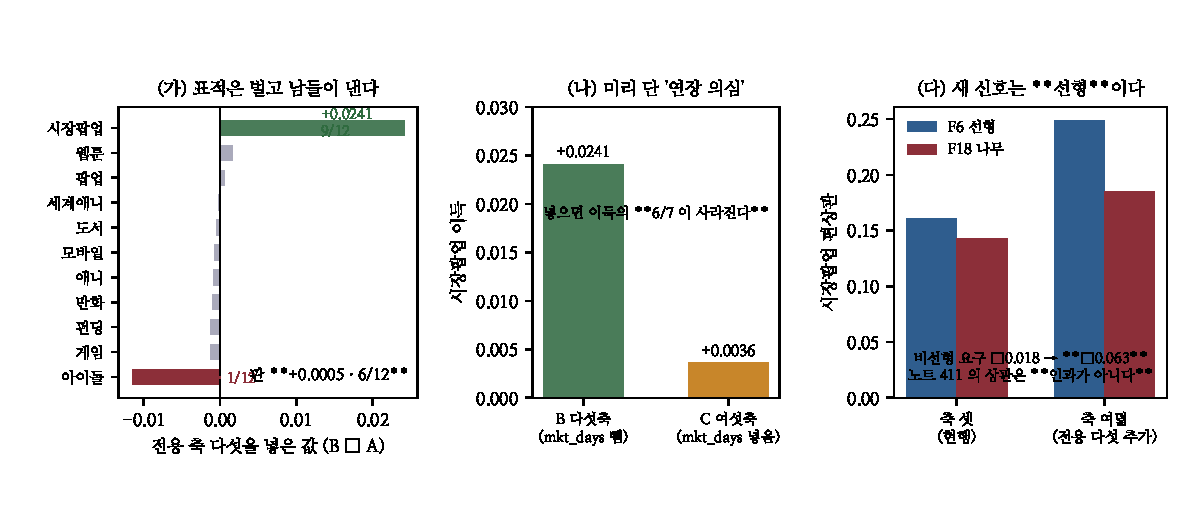
\includegraphics[width=\textwidth]{figs/fig412.pdf}
\caption{(가) 표적은 $+0.0241 \cdot 9/12$ 로 버는데 아이돌이 $-0.0115$ 로
낸다. (나) 미리 ``연장 의심''을 단 \texttt{mkt\_days} 를 넣으면 이득의
$6/7$ 이 사라진다. (다) 새 축의 신호는 선형이다 --- 그래서 비선형 요구가
더 음수가 됐다.}
\end{figure}

\end{document}
